\subsubsection*{Neuen Benutzer hinzufügen \faUsers}

Darüber hinaus kann er über den Button \jinline|Create| einen neuen Benutzer dem System anfügen. 
\abb \myRefGeneral{fig:AdminCreateUserImplement} zeigt die Eingabeform. 
Der Administrator muss hier den Benutzername und ein zufälliges Passwort wählen. 
Erstellte Benutzer durch den Administrator oder beim Zurücksetzen eines Passwortes erhalten als Sicherheitsfeature seitens der Datenbank \todo{Ref Niko, Ref Sicherheit FE} den Eintrag \jinline|isPasswordChangeRequiered|. 
Dies bedeutet, dass beim Einloggen der Benutzer auf die Seite zum Ändern des Passwortes geleitet wird und sich ansonsten nicht im System bewegen kann, bis er sein Passwort geändert hat. 

Dadurch wird Anforderung~\ref{Anf:A5}, die Pflicht zur Passwortänderung bei manueller Registrierung, erfüllt.

\begin{figure}[hp]
	\centering
	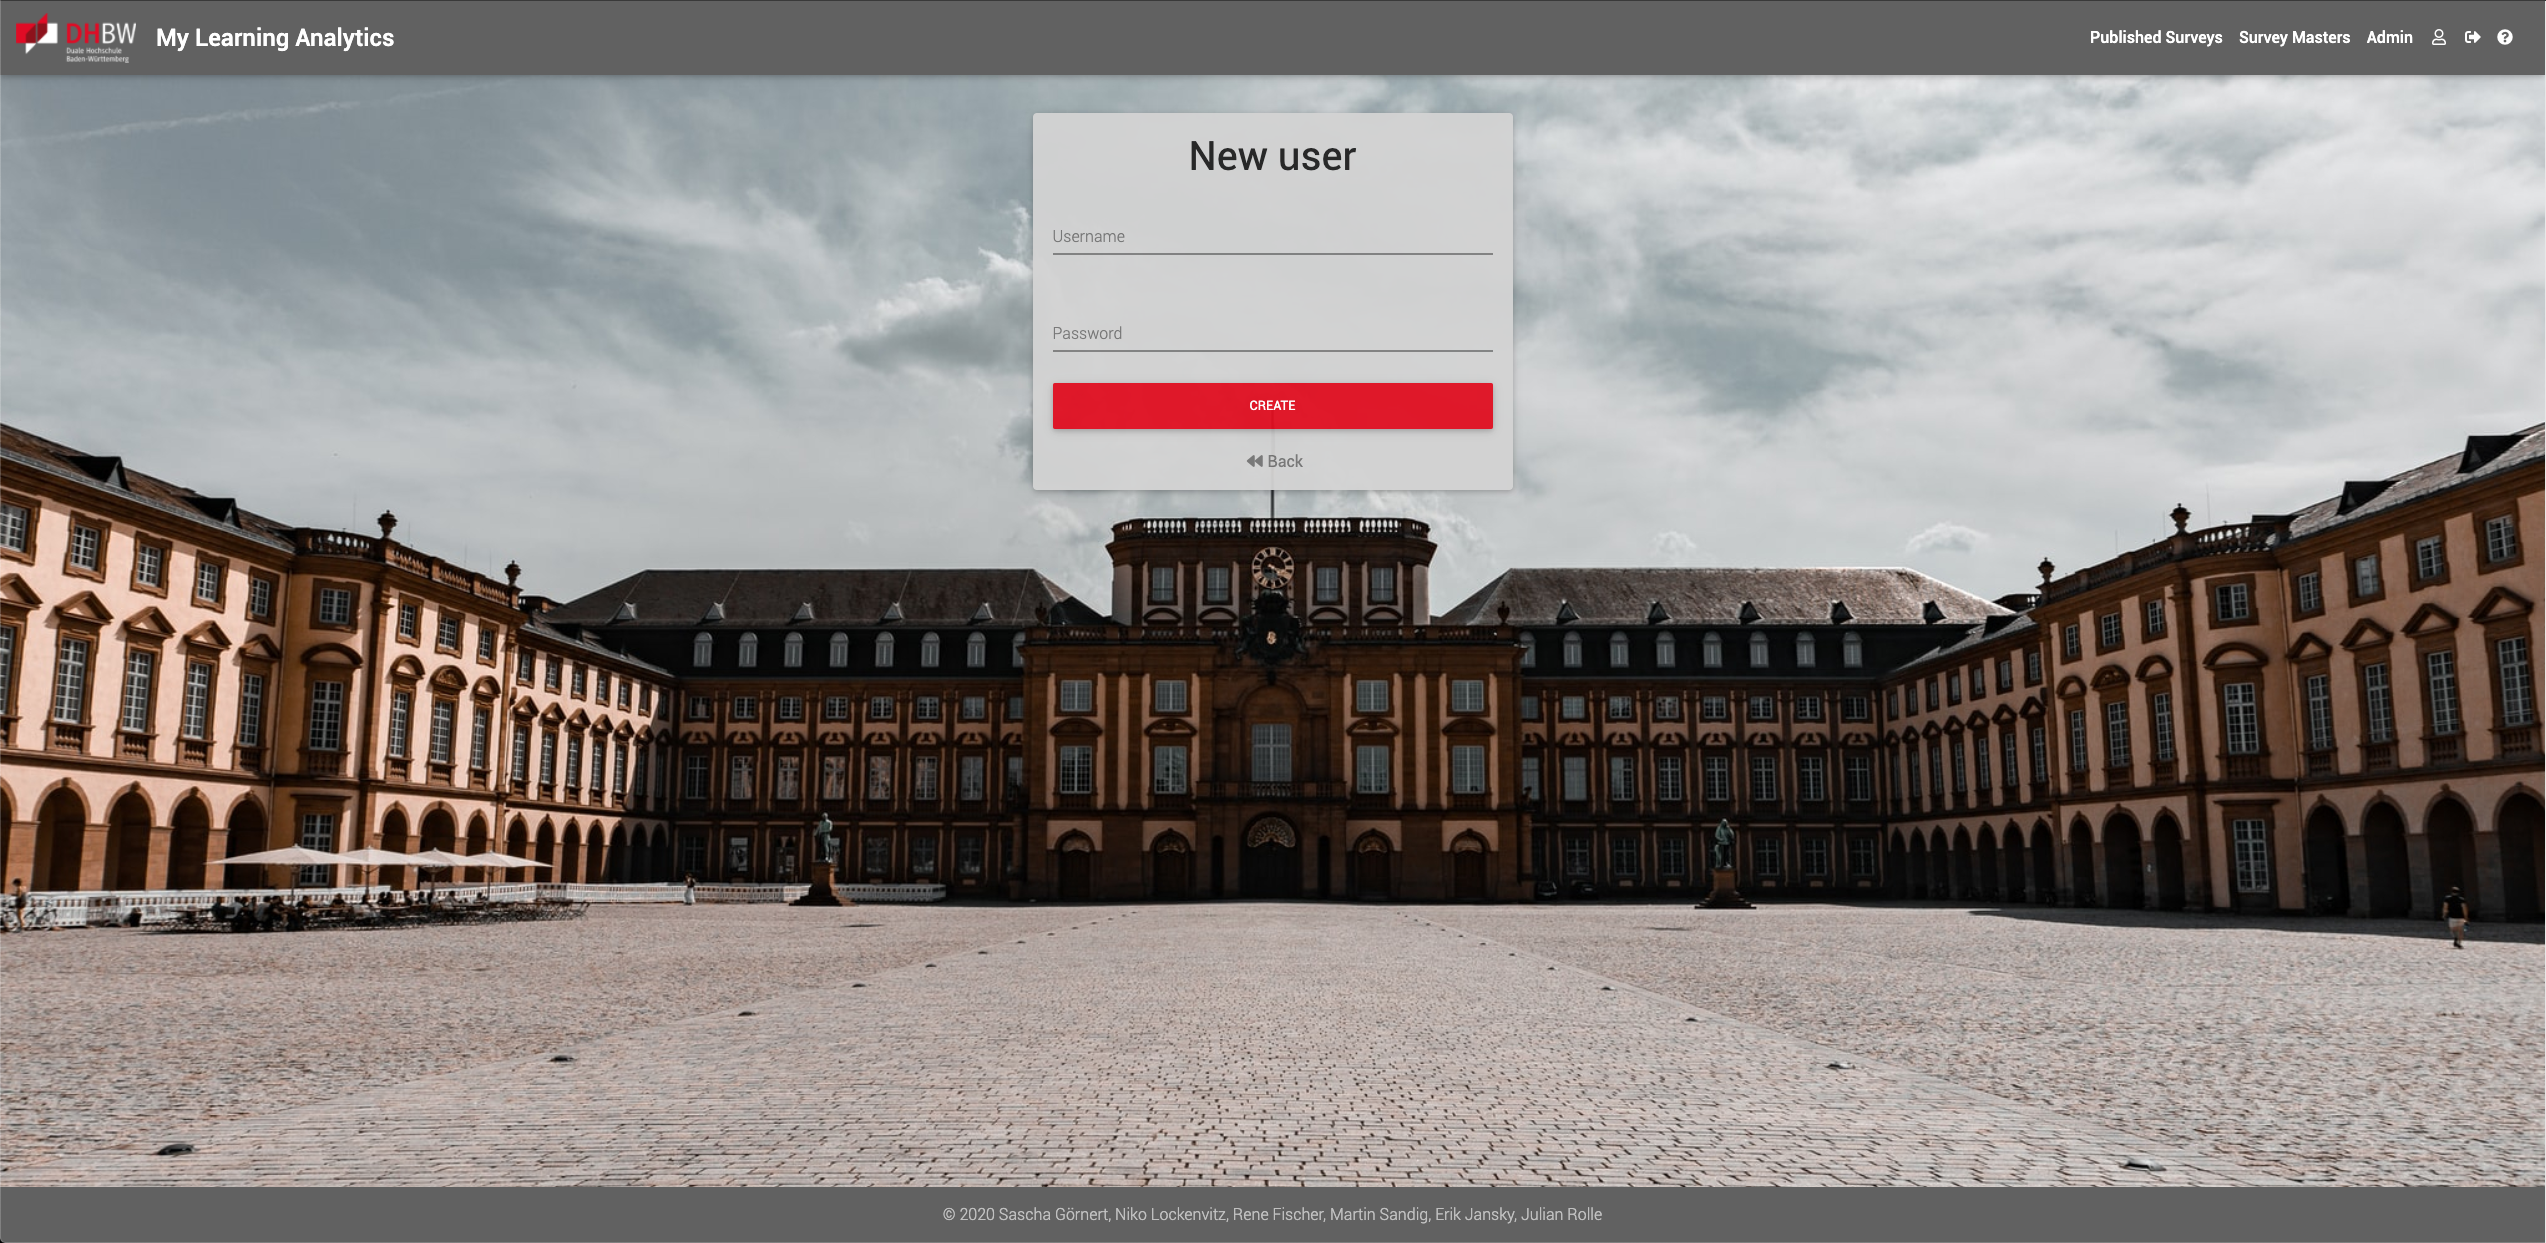
\includegraphics[width=0.95\textwidth, keepaspectratio]{img/client/AdminCreateUser.png}
	\captionsetup{justification=centering, format=plain}
	\caption[\acf{UI}: Neuen Benutzer der Anwendung hinzufügen]{\acf{UI}: Neuen Benutzer der Anwendung hinzufügen \\ \quelleScreenshot}
	\label{fig:AdminCreateUserImplement}
\end{figure}

